% Owner: Khanh. ~0.4 page. Source: paper_acl/sections/analysis.tex (7.2, 7.4)
\subsection{Why Fusion Helps}\label{sec:why}
\TODOK{Complementary errors: on ImageNet-R, PGM and the linear head disagree on 14\% of test images (linear right
5.8\%, PGM right 3.2\%, both wrong 5.4\%). Fig.~\ref{fig:frontier}: training-time changes only trade old classes for
new ones, fusion raises both. Do NOT reuse the old sentence ``uncalibrated sum +0.25/+0.44'' (different definition
from Table~\ref{tab:ablation}).}

\begin{figure}[t]
\centering
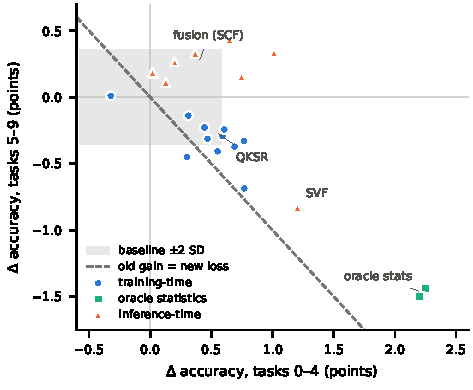
\includegraphics[width=0.6\textwidth]{figures/frontier.pdf}
\caption{Change of final accuracy on old (tasks 0--4) and new (tasks 5--9) halves, ImageNet-R seed 1993.
\TODOK{Rewrite the caption; shrink or drop the figure if pages run short.}}
\label{fig:frontier}
\end{figure}
